\chapter{Odašiljači iBeacon}

Odašiljači iBeacon su jeftini uređaji, niske potrošnje energije koji korištenjem BLE tehnologije obavještavaju obližnje uređaje o svojoj prisutnosti. 
Obližnji uređaji (poput mobilnih uređaja i tableta) mogu se pretplatiti na notifikacije odašiljača te mogu primati razne sadržaje (poput teksta, slika ili URL adresa) od njih. 
Krajem 2013. godine iBeacon tehnologiju patentirala je američka multinacionalna korporacija Apple Inc.
\\

Neki od zanimljivih načina primjene iBeacon tehnologije su u muzejima, trgovinama, bolnicama i ostalim ustanovama gdje se sadržaj mijenja ovisno o položaju u prostoriji. 
Posjetitelj muzeja može na mobilni uređaj ili tablet primiti sadržaj o objektu kojega trenutno promatra (npr. informacije o skulpturi ili slici), uz to, osoblje muzeja može pratiti koji su objekti najgledaniji i slično. 
U bolnici se može primijeniti tako da liječnik dobije sve podatke o pacijentu, od povijesti bolesti do trenutne dijagnoze, kada se približi njegovoj sobi ili krevetu. 
U trgovini se može iskoristiti tako da kupca obavijesti o predmetima na popustu u blizini. 
Također, iBeacon odašiljači mogu se iskoristiti i kao sustav plaćanja na sličan način kako se i NFC\footnote{\textit{Near field communication}, bežična tehnologija jako kratkog dometa korištena za komunikaciju između dva krajnja uređaja} tehnologija koristi (npr. beskontaktna plaćanja).
Ovo su samo najjednostavniji i najopćenitiji slučajevi gdje se iBeacon tehnologija može ukomponirati, broj načina korištenja tehnologije je ogroman.
\\

iBeacon se može konfigurirati tako da se sadržaj šalje samo kad se uređaj približi odašiljaču na određenu udaljenost. 
Pri tome su definirana tri parametra udaljenosti: neposredna (\textit{immediate}), mala (\textit{near}) i velika (\textit{far}) udaljenost. 
Neposredna udaljenost je do nekoliko centimetara, mala do nekoliko metara, dok je velika udaljenost iznad deset metara. 
Ove vrijednosti su aproksimativne jer ovisno o stvarnim uvjetima u kojima su odašiljači postavljeni signal može dosta varirati pa precizne vrijednosti nisu upotrebljive.
\\

Pošto je iBeacon tehnologija relativno nova, detaljna specifikacija nije javno dostupna stoga su gotovo svi proizvođači iBeacon odašiljača reverznim inženjerstvom otkrili značajan dio iBeacon Bluetooth profila.
\\
Kada je Apple predstavio iBeacon tehnologiju objavili su aplikaciju AirLocate pomoću koje se iPhone ili iPad koji podržava BLE može ponašati kao iBeacon odašiljač. 
Također, pomoću iste aplikacije moguće je podesiti sve parametre odašiljača. 
Kombinacijom te aplikacije pokrenute na nekom iPhone ili iPad uređaju i uređaja koji može snimati Bluetooth Low Energy pakete (poput računala sa ugrađenim Texas Instruments CC2540 čipom) istraživači uključujući i \citep
{radiusReverseEng} su došli do strukture \textit{advertising} paketa koja je prikazana u tablici \ref{tbl:iBeacon}.

\begin{table}[H]
\centering
\caption{Struktura \textit{advertising} paketa iBeacon odašiljača}
\label{tbl:iBeacon}
	\begin{tabular}{*{3}{c}}
	\hline 
	Bajt & Vrijednost & Opis \\ 
	\hline 
	1. & 02 & Duljina podataka - 2 bajta \\ 
	2. & 01 & Tip podataka - zastavice \\ 
	3. & X & LE i BR/ERD zastavice \\ 
	4. & 1A & Duljina podataka - 26 bajtova \\ 
	5. & FF & Podaci o proizvođaču \\ 
	6. & 4C & Podaci o proizvođaču - Apple \\ 
	7. & 00 & Podaci o proizvođaču - Apple \\ 
	8. & 02 & Tip podataka \\ 
	9. & 15 & Duljina podataka - 15 bajta \\ 
	10. & X & \textit{Proximity UUID} 1. bajt \\ 
	11. & X & \textit{Proximity UUID} 2. bajt \\ 
	12. & X & \textit{Proximity UUID} 3. bajt \\ 
	13. & X & \textit{Proximity UUID} 4. bajt \\ 
	14. & X & \textit{Proximity UUID} 5. bajt \\ 
	15. & X & \textit{Proximity UUID} 6. bajt \\ 
	16. & X & \textit{Proximity UUID} 7. bajt \\ 
	17. & X & \textit{Proximity UUID} 8. bajt \\ 
	18. & X & \textit{Proximity UUID} 9. bajt \\ 
	19. & X & \textit{Proximity UUID} 10. bajt \\ 
	20. & X & \textit{Proximity UUID} 11. bajt \\ 
	21. & X & \textit{Proximity UUID} 12. bajt \\  
	22. & X & \textit{Proximity UUID} 13. bajt \\ 
	23. & X & \textit{Proximity UUID} 14. bajt \\  
	24. & X & \textit{Proximity UUID} 15. bajt \\ 
	25. & X & \textit{Proximity UUID} 16. bajt \\ 
	26. & X & \textit{Major value} 1. bajt \\ 
	27. & X & \textit{Major value} 1. bajt \\ 
	28. & X & \textit{Minor value} 1. bajt \\  
	29. & X & \textit{Minor value} 2. bajt \\ 
	30. & X & RSSI na udaljenosti od 1m \\ 
	\hline 
	\multicolumn{3}{p{2pt}}X - vrijednosti ovise o postavkama konkretnog odašiljača
	\end{tabular}
\end{table}

Izuzev trećeg bajta sa LE (\textit{skraćeno od Low Energy}) i BR/ERD (\textit{skraćeno od Bluetooth Radio/Enhanced Data Rate}) zastavicama prvih devet bajtova svakog paketa su jednaki kod svakog odašiljača. 
Nakon toga slijedi šesnaest bajtova koji čine \textit{Proximity UUID\footnote{\textit{Universally unique identifier}}} parametar, dva bajta koji čine \textit{Major value} parametar, dva bajta koja čine \textit{Minor value} parametar te posljednji, trideseti, bajt koji sadrži RSSI\footnote{\textit{received signal strength indicator}, mjera jakosti primljenog signala} izmjeren na udaljenosti od jednog metra.vrijednost
\\
Konfigurabilni parametari \textit{Proximity UUID}, \textit{Major value} i \textit{Minor value} koriste se za identifikaciju pojedinog odašiljača. 
Preporuča se korištenje tih vrijednosti na način da \textit{Proximity UUID} bude nekakav globalni identifikator, a \textit{Major value} i \textit{Minor value} specifičniji identifikatori. 
Konkretno, \textit{Proximity UUID} može biti oznaka konkretnog trgovačkog lanca, \textit{Major value} oznaka konkretne trgovine, dok \textit{Minor value} može biti oznaka konkretne kategorije u trgovini.
\\
Posljednji bajt \textit{advertising} paketa sadrži RSSI izmjeren na udaljenosti od jednog metra od odašiljača. 
On se koristi kod određivanja udaljenosti od odašiljača. 
Pošto jakost signala na nekoj udaljenosti ovisi o okolini u kojoj je uređaj postavljen, radi pouzdanijeg određivanja relativne udaljenosti od odašiljača preporuča se prije početka korištenja odašiljača izmjeriti RSSI na udaljenosti od jednog metra te pohraniti tu vrijednost u sam odašiljač.

\section*{Kontakt.io Beacon}

Glavne značajke uređaja su odašiljanje podatkovnih paketa korištenjem BLE tehnologije te kompatibilnost sa svim uređajima koji podražavaju Bluetooth 4.0. 
Uz to, uređaji se mogu jednostavno klonirati i nadograditi, imaju visoku razinu sigurnosti te malu energetsku potrošnju.
\\
Pojedini uređaj ima nekoliko konfigurabilnih parametara: ime uređaja, \textit{Proximity UUID}, \textit{major} i \textit{minor} vrijednosti, \textit{transmisssion power level} te interval odašiljanja poruka.
\\
Uređaj napaja jedna CR2477 baterija s kojom uređaj može konstantno raditi više od 24 mjeseca \citep{kontaktDatasheet}. 
Raspon odašiljanja ovisi o snazi odašiljanja signala (parametar \textit{transmisssion power level}) te okolini u kojoj je odašiljač postavljen. 
Pri standardnoj (tvorničkoj) snazi odašiljanja iznosa \SI{-4}{dBm}, mobilni uređaj (ili bilo koji drugi uređaj sa podruškom za BLE) može prepoznati odašiljač do oko šest metara udaljenosti, dok na najjačoj snazi odašiljanja iznosa \SI{4}{dBm}, odašiljač se može prepoznati i na udaljenosti većoj od 20 metara.

\subsection*{Tehnička specifikacija}

Dimenzije odašiljača su $\SI{55}{mm} \times \SI{55}{mm} \times \SI{15}{mm}$ te on teži svega $23$ grama. 
Vanjski okvir je od ABS\footnote{Akrilonitril butadien stiren, izdržljiva plastika koja je pogodna za recikliranje} plastike, a uređaj napaja zamjenjiva CR2477 baterija s kojom odašiljač može raditi više od 24 mjeseca. 
Prema \citep{kontaktTehnical} vrijeme rada može se dodatno povećati na čak šest godina ukoliko se smanje jakost odašiljanja i interval odašiljanja poruka.
\\
Ostale karakteristike odašiljača su:
\begin{itemize}
    \item Bluetooth Smart multiprotocol SOC\footnote{sustav na čipu \engl{System on a chip}} IC\footnote{integrirani krug \engl{integrated circuit}} kojega proizvodi Nordic Semiconductors
    \item $32$-bitni ARM Cortex M0 procesor
    \item $\SI{256}{kB}$ flash memorije
    \item $\SI{16}{kB}$ RAM memorije
    \item Jakost odašiljanja u rasponu od $\SI{-30}{dBm}$ do $\SI{+4}{dBm}$
    \item Dozvoljene brzine prijenosa: $\SI{250}{kBs}$, $\SI{1}{Mbs}$ i $\SI{2}{Mbs}$
\end{itemize}

\begin{figure}[H]
    \centering
    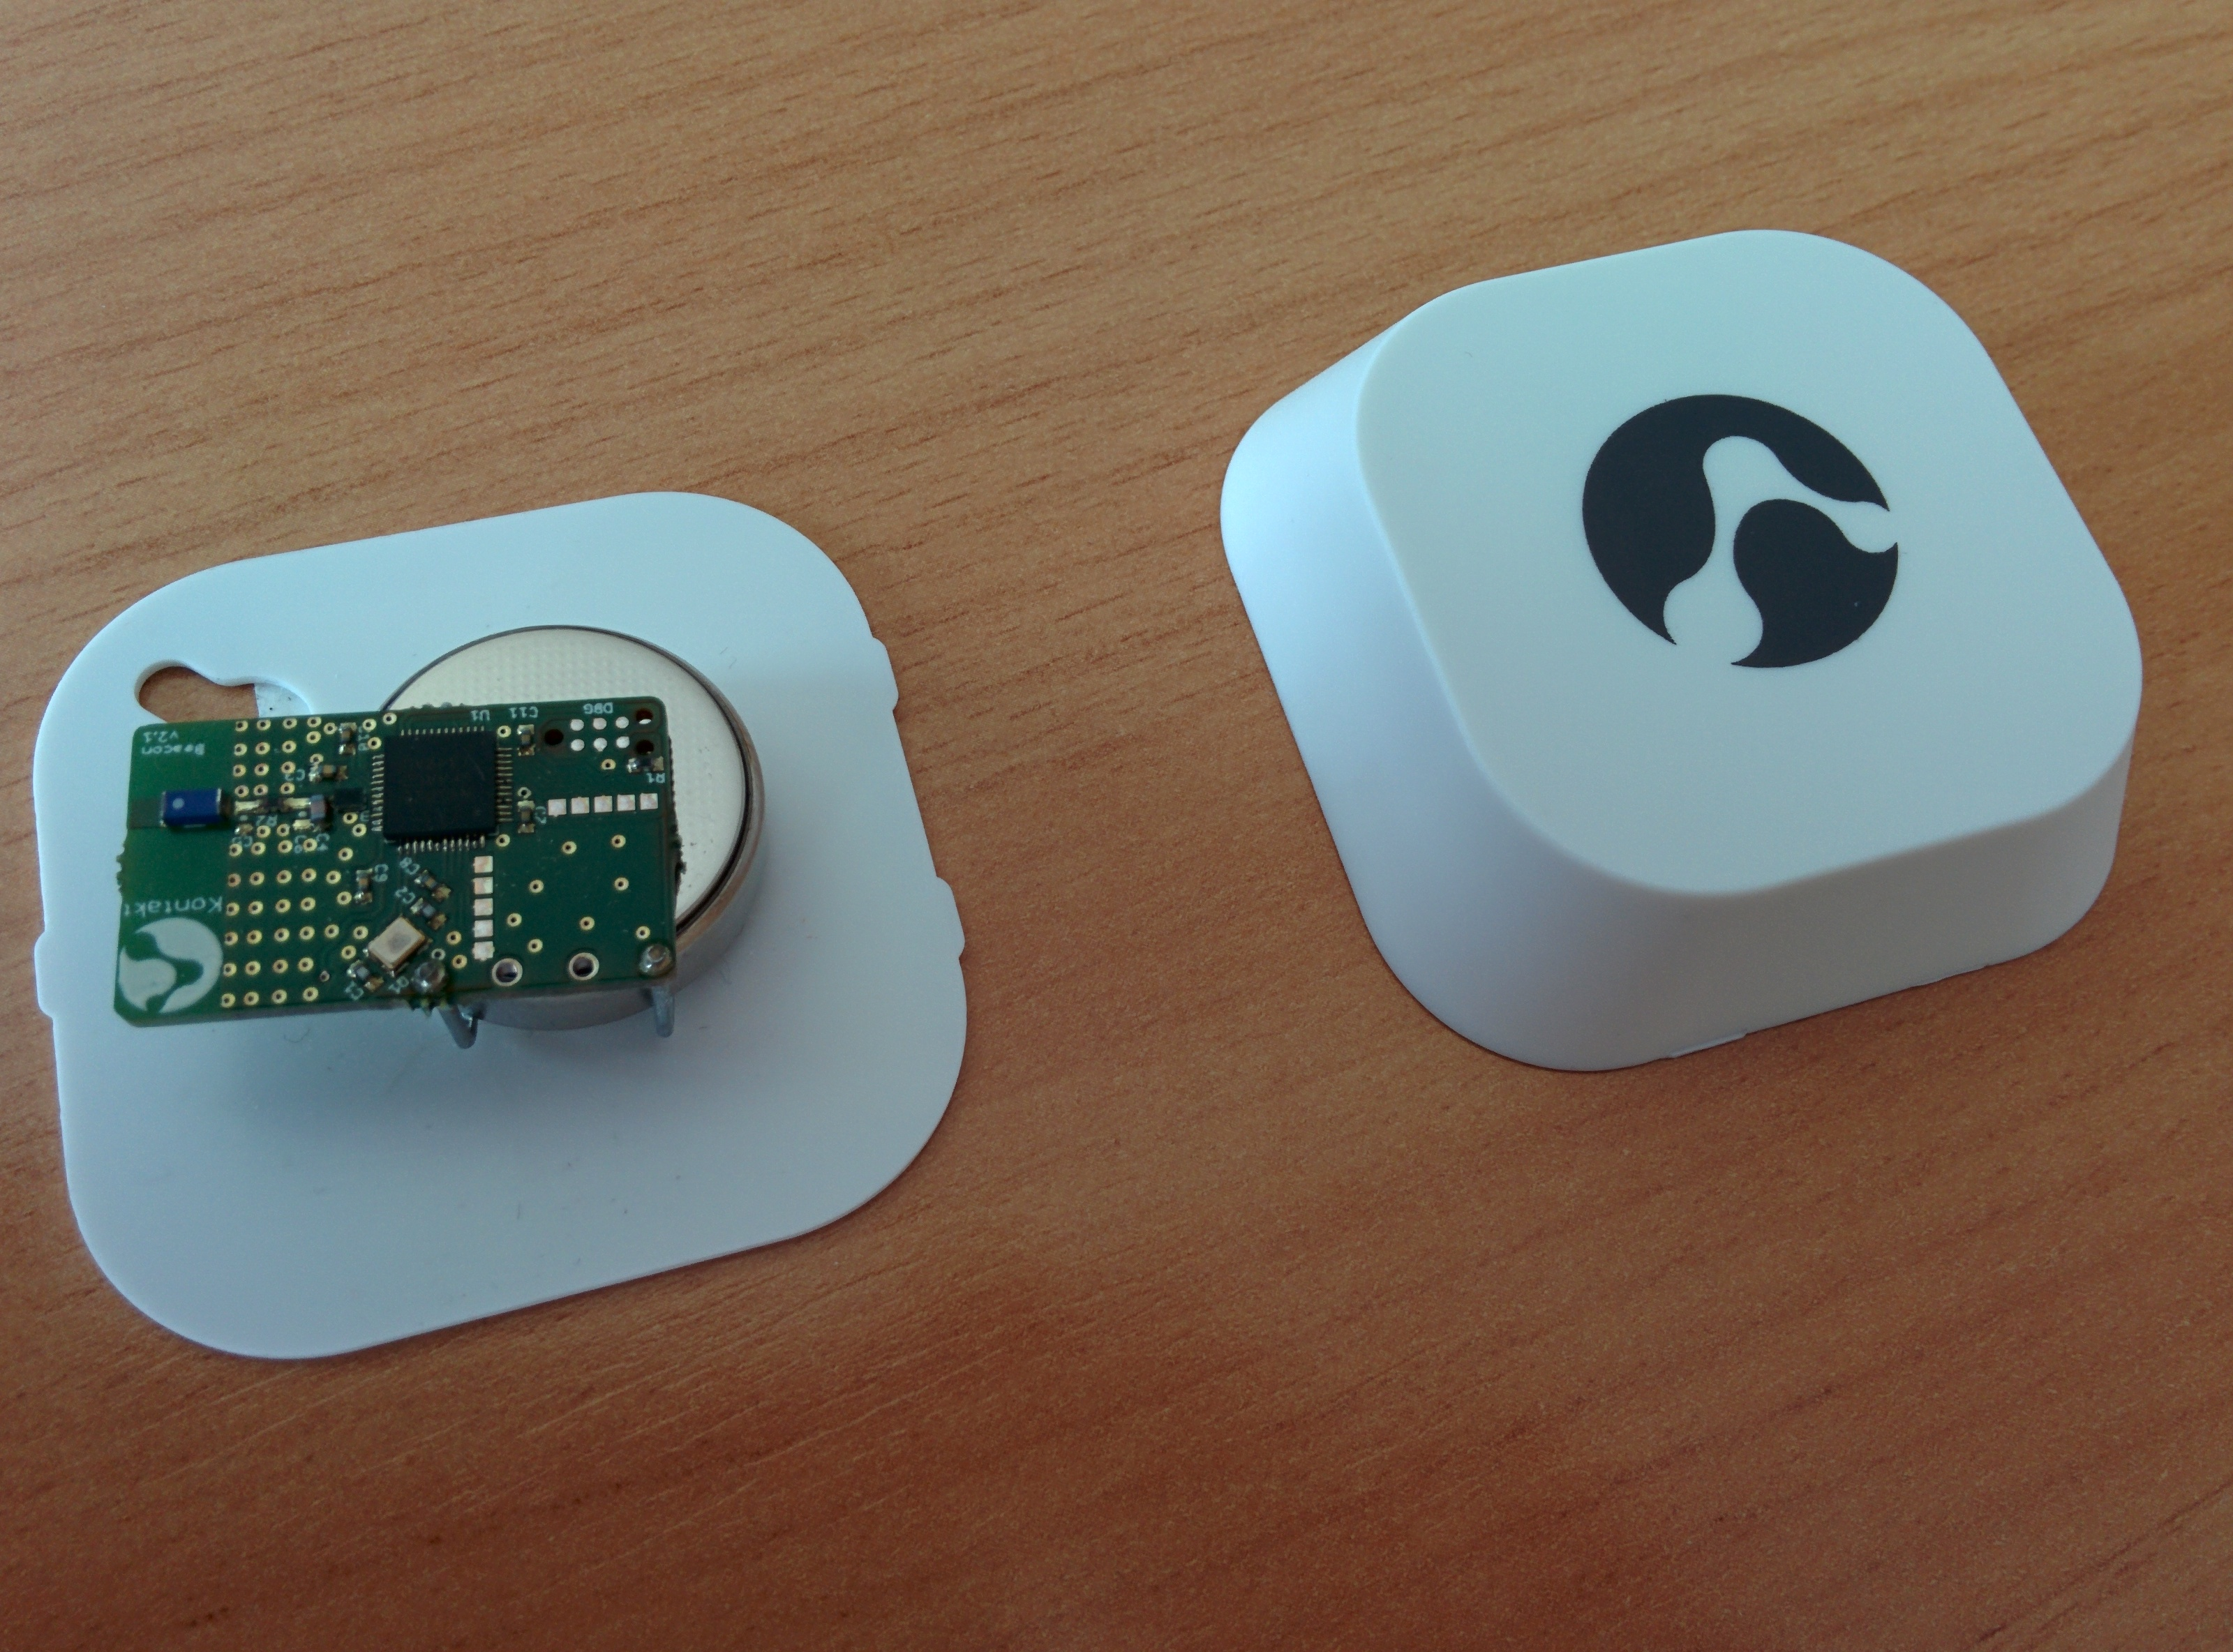
\includegraphics[scale=0.1]{pictures/IMG_20140505_095855}
    \caption{Kontakt.io iBeacon odašiljač}
\end{figure}

Dozvoljene vrijednosti jakosti odašiljanja su: $\SI{-30}{dBm}$, $\SI{-20}{dBm}$, $\SI{-16}{dBm}$, $\SI{-12}{dBm}$, $\SI{-8}{dBm}$, $\SI{-4}{dBm}$, $\SI{0}{dBm}$ i $\SI{4}{dBm}$.


\subsection*{Struktura paketa}
Uređaj odašilje dvije vrste paketa podataka: \textit{advertising} i \textit{scan response}.
\\
Tokom rada uređaj kontinuriano odašilje \textit{advertising} pakete i na taj obavještava okolne uređaje o svojoj prisutnosti. 
Drugi tip paketa, \textit{scan response} paket, šalje se odmah nakon \textit{advertising} paketa i sadrži dodatne informacije o odašiljaču, poput imena odašiljača, stanja baterije i slično.
\\

Struktura \textit{advertising} paketa odgovara strukturi iBeacon \textit{advertising} paketa navedenog u tablici \ref{tbl:iBeacon}, dok je struktura \textit{scan response} paketa navedena u tablici \ref{tbl:scanResponse}.
\\
%Prvih devet bajtova paketa su unaprijed poznate konstante (poput informacije o proizvođaču). Njih slijedi šesnaest bajtova koji čine proximity UUID, dva bajta za \textit{major} vrijednost, dva bajta za \textit{minor} vrijednost, a posljednji bajt predstavlja RSSI vrijednost (engl. \textit{Recived Signal Strength Indication}) izmjeren jedan metar od iBeacon uređaja.

\begin{table}[H]
    \centering
    \caption{Struktura \textit{scan response} paketa}
    \label{tbl:scanResponse}
    \begin{tabular}{ccc}
    \hline 
    Bajt & Vrijednost & Opis \\ 
    \hline 
    1. & 08* & Duljina podataka - 8 bajta \\ 
    2. & 09 & Tip podatka - Complete Local Name \\ 
    3. & 4B* & Lokalno ime uređaja \\ 
    4. & 6F* & Lokalno ime uređaja \\ 
    5. & 6E* & Lokalno ime uređaja \\ 
    6. & 74* & Lokalno ime uređaja \\ 
    7. & 61* & Lokalno ime uređaja \\ 
    8. & 6B* & Lokalno ime uređaja \\ 
    9. & 74* & Lokalno ime uređaja \\ 
    10. & 02 & Duljina podataka - 2 bajta \\ 
    11. & 0A & Tip podataka - Tx Power Value \\ 
    12. & F4 & Tx Power Value \\ 
    13. & 0A & Duljina podataka - 10 bajta \\ 
    14. & 16 & Tip podataka - service data \\ 
    15. & 0D & Service UUID 1. bajt \\ 
    16. & D0 & Service UUID 2. bajt \\ 
    17. & X & Identifikator odašiljača 1. bajt \\ 
    18. & X & Identifikator odašiljača 2. bajt \\ 
    19. & X & Identifikator odašiljača 3. bajt \\ 
    20. & X & Identifikator odašiljača 4. bajt \\ 
    21. & X & Firmware version 1. bajt \\ 
    22. & X & Firmware version 2. bajt \\ 
    23. & X & Razina baterije \\ 
    \hline
    \multicolumn{3}{p{2pt}}X - vrijednosti ovise o postavkama konkretnog odašiljača \\
    \multicolumn{3}{p{2pt}}* - varijabilne duljine, ovisi o duljini postavljenog imena odašiljača (max. 15 bajtova)
    \end{tabular} 
\end{table}